% !TEX encoding = UTF-8 Unicode
% !TEX root = SystemTemplate.tex

\documentclass{book}
% !TEX root = SystemTemplate.tex

\usepackage[width=6.5in, height=9.2in, top=1.0in, papersize={8.5in,11in}]{geometry}
\usepackage[pdftex]{graphicx}
%\usepackage{draftwatermark}
\usepackage{amsmath}
\usepackage{amsthm}
\usepackage{amssymb}
%\usepackage{txfonts}
\usepackage{textcomp}
%\usepackage{amsthm}

\usepackage[all]{xy}
\usepackage{fancyhdr}
\pagestyle{fancy}
\usepackage{hyperref}
\usepackage{verbatim}
\usepackage{algorithm}
\usepackage{algorithmic}
\usepackage{array}
\usepackage{color}
\usepackage{listings}
\lstset{language=c,frame=ltrb,framesep=5pt,basicstyle=\normalsize,
 keywordstyle=\ttfamily\color{DarkRed},
identifierstyle=\ttfamily\color{DarkBlue}\bfseries,
commentstyle=\color{OliveGreen},
stringstyle=\ttfamily,
showstringspaces=false,tabsize = 3}
\usepackage{calc}
\usepackage{doxygen}
\usepackage[utf8]{inputenc}
\usepackage{makeidx}
\usepackage{multicol}
\usepackage{multirow}
\usepackage[table]{xcolor}

\definecolor{color02}{rgb}{0.18,0.35,0.59}
\definecolor{color03}{rgb}{0.44,0.59,0.82}
\definecolor{color06}{rgb}{0.35,0.35,0.35}


\newtheorem{summary}{Summary:}
\newtheorem{example}{Example:}


\definecolor{OliveGreen}{cmyk}{0.64,0,0.95,0.40}
\definecolor{DarkBlue}{cmyk}{0.76,0.76,0,0.20}
\definecolor{DarkRed}{cmyk}{0,1,1,0.45}


\def      \RR             {{\mathbb R}} 
\def      \DS            {\displaystyle} 

\setlength{\oddsidemargin}{0mm} 
\setlength{\evensidemargin}{0mm} 

%\SetWatermarkLightness{0.975}
%\SetWatermarkScale{6}
%\SetWatermarkText{\includegraphics{test.png}}

\pagestyle{fancy}
\renewcommand{\chaptermark}[1]{\markboth{#1}{}}
\renewcommand{\sectionmark}[1]{\markright{\thesection\ #1}}
\fancyhf{}
\fancyhead[LE,RO]{\bfseries\thepage}
\fancyhead[LO]{\bfseries\rightmark}
\fancyhead[RE]{\bfseries\leftmark}
\fancyfoot[LE,RO]{Confidential and Proprietary}
%\renewcommand{\headrulewidth}{0.5pt}
%\renewcommand{\footrulewidth}{0pt}
%\addtolength{\headheight}{0.5pt}
%\setlength{\footskip}{0mm}
%\renewcommand{\footruleskip}{0pt}


\definecolor{MSBlue}{rgb}{.204,.353,.541}
\definecolor{MSLightBlue}{rgb}{.31,.506,.741}
\definecolor{MSBlue1}{rgb}{0.18,0.35,0.59}
\definecolor{MSBlue2}{rgb}{0.44,0.59,0.82}
\definecolor{MSBlue3}{rgb}{0.35,0.35,0.35}


\usepackage{titlesec}
\titleformat{\chapter}[display]
{\normalfont\bfseries\color{MSBlue1}}    %\normalfont\bfseries\filcenter}
{\LARGE\thechapter}
{1ex}
{\titlerule[2pt]
\vspace{2ex}%
\LARGE}
[\vspace{1ex}%
{\titlerule[2pt]}]

\definecolor{MSBlue}{rgb}{.204,.353,.541}
\definecolor{MSLightBlue}{rgb}{.31,.506,.741}
\definecolor{MSBlue1}{rgb}{0.18,0.35,0.59}
\definecolor{MSBlue2}{rgb}{0.44,0.59,0.82}
\definecolor{MSBlue3}{rgb}{0.35,0.35,0.35}

%\titleformat*{\section}{\Large\bfseries\sffamily\color{MSBlue}}
%\titleformat*{\subsection}{\large\bfseries\sffamily\color{MSLightBlue}}
%\titleformat*{\section}{\Large\bfseries\color{MSBlue1}}
%\titleformat*{\subsection}{\large\bfseries\color{MSBlue2}}

\titleformat*{\section}{\Large\bfseries\color{MSBlue}}
\titleformat*{\subsection}{\large\bfseries\color{MSLightBlue}}
\titleformat*{\subsubsection}{\large\bfseries\color{MSBlue3}}
\setcounter{secnumdepth}{3}
\renewcommand{\thesubsubsection}{\thesubsection.\alph{subsubsection}}

 % This sets the format.

% Add your title page contents here 
\title{{\color{MSBlue1} \rule{\linewidth}{0.5mm}}\\[2mm] {\huge \bfseries \color{MSBlue1} Product Title }\\[-1mm] {\color{MSBlue1}\rule{\linewidth}{0.5mm}} \\  \vfill
{\LARGE \bfseries \color{MSBlue2} Testing System Project }\\  \vfill 
{\color{MSBlue1} LaTex Samurai} }
\author{\color{MSBlue1}  Julain Brackins \and \color{MSBlue1} Jonathan Dixon \and  \color{MSBlue1} Hafiza Farzami }
\date{\color{MSBlue1} \today}


\begin{document}
\frontmatter
\maketitle


\tableofcontents
\listoffigures
\listoftables
\listofalgorithms


% !TEX root = SystemTemplate.tex

\chapter{Mission}

The mission statement for this project is to create a test suite designed to compile and run C++ projects with various numerical test cases. This project will run on many student folders and allows for basic test case generation.  % add mission statement to mission.tex
% !TEX root = SystemTemplate.tex

\chapter{Document Preparation and Updates}

Current Version [1.0.0]
\vspace*{5mm}

{\color{MSBlue3}
\noindent
\textit{Prepared By:}\\
\textit{Hafiza Farzami}\\
%\textit{Team Member \#2}\\
%\textit{Team Member \#3}
}

\vfill
\noindent
{\color{color02} \textit{\textbf{Revision History}}}\\
\begin{tabular}{|>{\raggedright}p{1.5cm}|>{\raggedright}p{3cm}|>{\raggedright}p{1.5cm}|>{\raggedright}p{9cm}|}
\hline
\textit{\textbf{Date}} &  \textit{\textbf{Author}} & \textit{\textbf{Version}} & \textit{\textbf{Comments}}\tabularnewline
\hline
 \textit{\textbf{2/17/14}} & \textit{Hafiza Farzami} & \textit{1.0.0} & \textit{Initial version}\tabularnewline
\hline
%\textit{\textbf{3/4/12}} & \textit{Team Member \#3} & \textit{1.1.0} & \textit{Edited version}\tabularnewline
%\hline
 &  &  & \tabularnewline
 \hline
 &  &  & \tabularnewline
\hline
 &  &  & \tabularnewline
\hline
 &  &  & \tabularnewline
\hline
 &  &  & \tabularnewline
\hline
\end{tabular}
\vfill



 
\mainmatter

%%  Add to the following chapters

% !TEX root = SystemTemplate.tex

\chapter{Overview and concept of operations}

This report covers the project overview, user stories, backlog, design and implementation, development environment, deployment, and documentation for the testing project. 


\section{Scope}
This section gives a brief overview of the system.


\section{Purpose}
The purpose of this program is to run {\tt .cpp} files with given test files, and grade them. 


\subsection{Traversing Subdirectories}
Traversing subdirectories is one of the main components of this system. The program runs a {\tt .cpp} file using test files, and the test files are stored in the current and all the subdirectories.  

\subsection{Running the Program Using Test Cases}
The software was designed in the Linux environment provided to the group by the university. 
 

\section{Systems Goals}
The goal of this system is to grade a {\tt .cpp} file just by typing {\tt grade <filename>.cpp}. The product is built to test the {\tt .cpp} file with all the given {\tt .tst} test files in the current directory and all the subdirectories, and compare the results to the corresponding {\tt .ans} files.  

\section{System Overview and Diagram}
Here is a flow diagram showing the implementation process:

\begin{figure}[tbh]
\begin{center}
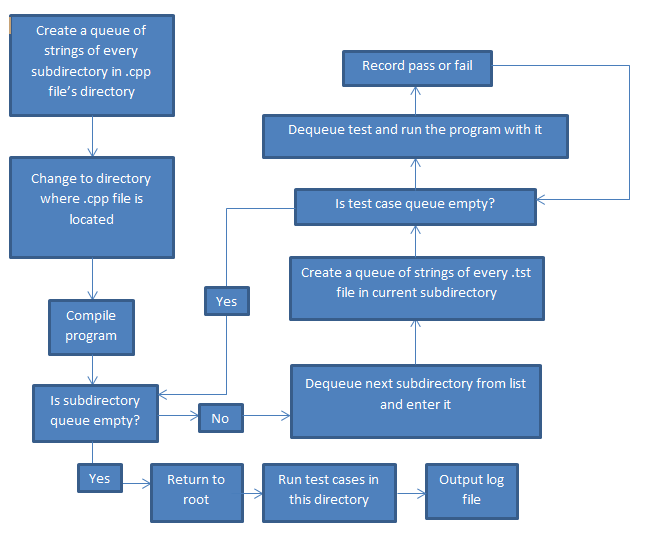
\includegraphics[width=0.75\textwidth]{./flowDiagram}
\end{center}
\caption{System Diagram \label{systemdiagram}}
\end{figure}





% !TEX root = SystemTemplate.tex


\chapter{Project Overview}
%This section provides some housekeeping type of information with regard to the 
%team, project, etc. 



\section{Team Members and Roles}

\begin{itemize}
  \item Ben Sherman - Product Owner
  \item James Tillma - Scrum Master
  \item Anthony Morast - Technical Lead  
\end{itemize}


\section{Project  Management Approach}
The aproach taken to manage this project is {\tt scrum}. The project is broken into tasks to be completed over two weeks sprint. The tasks are listed in {\tt Spring Backlog} in trello. During the sprint, the team meets for ten minutes scrum meetings to explain their progress, next steps, and impediments. 


\section{Phase  Overview}
Once a team member starts a given task, then the task is moved from {\tt Spring Backlog} to {\tt In Progress}. A done task is then moved to {\tt Ready for Testing} tab. After a completed task is tested, it is stamped as {\tt Complete}. Then the member moves to the next task. After each sprint the tasks are moved from complete to {\tt Product Backlog}

 

% !TEX root = SystemTemplate.tex
\chapter{User Stories, Backlog and Requirements}
\section{Overview}


This section covers user stories, backlog and requirements for the system.  





\subsection{Scope}

This document contains stakeholder information, 
initial user stories, requirements, proof of concept results, and various research 
task results. 



\subsection{Purpose of the System}
The purpose of the product is to grade a {\tt <filename>.cpp} file by running test files and comparing the results to answer files, and assigning percentage grade. 


\section{ Stakeholder Information}


This section would provide the basic description of all of the stakeholders for 
the project.

\subsection{Customer or End User (Product Owner)}
Jonathan Dixon is the product owner in this project, who is in contact with the scrum master and technical lead regarding the backlog. 

\subsection{Management or Instructor (Scrum Master)}
Hafiza Farzami is the scrum master, who breaks the project into smaller tasks, and is in touch with both product owner and technical lead.

%\subsection{Investors}
%Are there any?  Who?  What role will they play? 


\subsection{Developers --Testers}
Julian Brackins is the technical lead for Sprint 1, and is in contact with both Dixon and Farzami regarding the requirements during scrum meetings and through trello notes. 



\section{Business Need}
This product is essential for grading computer science programs focused on numerics. All the user have to do is have test cases and expected results in the directory that the {\tt <filename>.cpp} file is in and any of the subdirectories, and run the {\tt grade.cpp} program. It saves a lot of time, and is efficient. 

\section{Requirements and Design Constraints}
Use this section to discuss what requirements exist that deal with meeting the 
business need.  These requirements might equate to design constraints which can 
take the form of system, network, and/or user constraints.  Examples:  Windows 
Server only, iOS only, slow network constraints, or no offline, local storage capabilities. 


\subsection{System  Requirements}
This product runs on Linux machines. 


\subsection{Network Requirements}
This software does not require internet connection. 


\subsection{Development Environment Requirements}
There are not any development environment requirements.


\subsection{Project  Management Methodology}
The method used to manage this project is {\tt scrum}. The scrum master met with the product owner, and broke the tasks down to the technical lead. The team meets for ten minutes long scrum meetings to go over the progress, next steps, and impediments. 
 
\begin{itemize}
\item Trello is used to keep track of the backlogs and sprint status
\item Everyone has access to the Sprint and Product Backlogs
\item This project will take three Sprints
\item Each Sprint is two weeks long
\item There are no restrictions on source control 
\end{itemize}

\section{User Stories}
This section contains the user stories regarding functional requirements and how the team broke them down.




\subsection{User Story}
Write an automatic testing system. By Wednesday, your team should have a list of questions for me (the customer) on exactly what I require. Think CS150/250/300 programs - not major software.

\subsubsection{User Story Breakdown \#1}

The purpose of the program is to grade a student's file, comparing it to multiple test case files. It'll be called like this: {\tt grade <filename>.cpp}. It will grade the file, looking through the current directory for any {\tt .tst} files, which will contain the test cases. We must compile the program, which is in C++. 

It is understood that all inputs will be valid (no error checking, program won't crash, etc...). The program will be tested on numeric computations. If it uses files, they'll be {\tt input.txt} and {\tt output.txt}. {\tt <filename>.log} will contain the results of each test case.

The idea is to grab the test case, copy it to input.txt, run the program, compare outputs, and put results into the log file. {\tt .tst} files will have a test case followed by a blank line, followed by expected results.

\subsubsection{User Story Breakdown \#2}
A student submits a program.  That program is placed into a directory that forms the root of the directory tree related to that program.  All the instructors and teacher's assistant will have the ability to write test cases (called case\#.tst and the accompanying file case\#.ans).  There are no restrictions on where those files can be located except that they will be at the level of the .cpp file or below.  For example. Manes might have a subdirectory where he puts his test cases.  His TAs might have subdirectories under the Manes subdirectory where they put their test cases.  Manes might just make the directory but not put any test cases in it just so his TAs have a place to put theirs (in subdirectories).  I want to say 
test quadratic
and have your program find all the applicable test cases (with the accompanying answer files), run the tests, log the results, and provide a summary.  I want to be able to fix problems and rerun the test without losing the original log file.  Append the date so I can tell them apart.


% !TEX root = SystemTemplate.tex
\chapter{Design  and Implementation}
 This section describes the design details for the overall system as well as individual major components. As a user, you will have a good understanding of the implemetation details without having to look into the code. Note that the
 code to generate test cases is only run if there is a -g cammond line switch is specified after the directory to test is entered.

 Here is an overview of the algorithm:

\begin{itemize}
  \item Determine if there is a .cpp file in the root directory, if so it is used to generate test cases
  \item Create a vector of every subdirectory in program folder
  \item Change to directory where student subdirectories are located
  \item Step through each directory in the directory vector and determine if it contains tests or student source code
  \item Create a vector containing the name each student's source and one containing the path to their source code
  \item Create a vector of all the test cases
  \item While the source code vector is not empty
  \item Compile the program
  \item Determine if the student passes the critical test cases, if not stop testing
  \item Run code against tests in the test vecotor
  \item Count whether the program passed or failed test case
  \item Change back to home directory (where program is located)
  \item Create a queue of every .tst file in home directory
  \item While test case queue is not empty:
  \item Dequeue first test case in queue
  \item Run program using that test case
  \item Count whether the program passed or failed test case
  \item Write log file containing percentage of tests passed and final grade
  \item Write students results to summary file
\end{itemize}


\section{Traversing Subdirectories }

\subsection{Technologies  Used}
The dirent.h library is used for traversing subdirectories.

\subsection{Design Details}

\begin{lstlisting}

bool change_dir(string dir_name)
{
    string path;
    if(chdir(dir_name.c_str()) == 0) 
    {
        path = get_pathname();
        return true;
    }
    return false;
}

bool is_dir(string dir)
{
    struct stat file_info;
    stat(dir.c_str(), &file_info);
    if ( S_ISDIR(file_info.st_mode) ) 
        return true;
    else 
        return false;
}
\end{lstlisting}

\section{Running the Program Using Test Cases }

\subsection{Technologies  Used}
The software was designed in the Linux Environment.


\subsection{Design Details}


\begin{lstlisting}
int run_file(string cpp_file, string test_case) //case_num
{
    //create .out file name
    string case_out(case_name(test_case, "out"));

    //set up piping buffers
    string buffer1("");
    string buffer2(" &>/dev/null < ");
    string buffer3(" > ");

    // "try using | "
    //construct run command, then send to system
    //./<filename> &> /dev/null  < case_x.tst > case_x.out
    buffer1 += cpp_file + buffer2 + test_case + buffer3 + case_out;
    system(buffer1.c_str());

    //0 = Fail, 1 = Pass
    return result_compare(test_case);
}
\end{lstlisting}



% !TEX root = SystemTemplate.tex

\chapter{System  and Unit Testing}

Testing was first done on small parts of the program, and as we added more, we tested larger parts of the program.

\section{Overview}
In general, we began testing on a lower level by testing our 
capabilities for rerouting input and output. Once we managed that,
we moved on to comparing output files to the test case files. Once Dr. 
Logar released the test cases, we created a function to confirm directory 
traversals. Then, when we combined the two, our program functioned correctly
and we were able to add the finishing touches.



\section{Dependencies}
No dependencies.


\section{Test Setup and Execution}
\subsection{Studenfile:///C:/Users/Ben/SkyDrive/Documents/2014 Spring/SoftEng/Sprint2/SystemDiagram.vsdxt Grading}
The student grading section involves
\begin{itemize}
\item Crawling through student directories.
\item Running each students source code on the test cases.
\end{itemize}
The product was tested on the customer supplied example class directory and class directories where created to for further testing.

\paragraph{} Below is a list of the individual directories that where used in testing as well as the difference between them that tested aspects of the product.

\paragraph{Customer Test CSC\_150 Class Directory}
This product test demonstrates the products ability to test a class without any critical test cases multiple directories. It also demonstrates automatic test case generation.
\begin{verbatim}
Customer Test CSC_150 Class Directory:
  Students:
    bad_student_1 Fails some test cases
    bad_student_2 Fails some test cases
    student_3 Passes all test cases
    student_4 Passes all test cases
    
  Multiple directories containing tests
  No critical test cases
  Golden Source Code: average.cpp
  directories containing useless files
\end{verbatim}

\paragraph{Test Directory 1}
This created test demonstrates the products ability to fail a student if they do not pass a critical test case. It also demonstrates automatic test case generation.
\begin{verbatim}
Test Directory 1:
  Students:
    Alex_Johnson
    Bob
    Francis
    John
    
  Critical and normal test cases
  Golden Source Code: max_3.cpp
\end{verbatim}

\paragraph{Test Directory 2}
This created test demonstrates the programs ability fail a student if they do not pass a critical test case; it demonstrates the ability of the product to find test cases in subdirectories; finally it demonstrates the products ability to allow test case generation only when a golden source code is available.
\begin{verbatim}
Test Directory 2:
  Students:
    student_1 Fails critical
    student_2 Fails critical
    student_3 Passes all test cases
    student_4 Passes all test cases
    student_5 Passes all test cases
    student_6 Passes all test cases
    student_7 Passes all test cases

  Test case subdirectories
  Critical and normal test cases
  Golden Source Code: none
\end{verbatim}



% !TEX root = SystemTemplate.tex
\chapter{Development Environment}
The basic purpose for this section is to give a developer all of the necessary 
information to setup their development environment to run, test, and/or develop. 


\section{Development IDE and Tools}
Code was modified through the use of gedit and the text editor available on the git website.

\section{Source  Control}
Git was used for source control. It was set up on GitHub, and can be accessed via the command
	
	git connect https://github.com/jbrackins/CSC470.git

\section{Dependencies}
An internet connection to access the Git will be necessary.

\section{Build  Environment}
The program may be built using the g++ compiler on linux.



% !TEX root = SystemTemplate.tex

\chapter{Release -- Setup -- Deployment}


\section{Deployment Information and Dependencies}
This program has no dependiencies other than it needs to be compiled and run within a linux environment. 



\section{Setup Information}
The program is built with the g++ compiler on linux. The program can also be built by typing {\tt make}.



\section{System  Versioning Information}
The program will be versioned depending on the current Agile sprint. The current sprint version is 2.0.

% !TEX root = SystemTemplate.tex

\chapter{User Documentation}

%\newpage   %% 
%%  The user guide can be an external document which is included here if necessary ...
%%  a single source is the way to go.

\section{User Guide}

This product is to make it easy for you to grade multiple computational computer program written in C++ language. In order to benefit from this product, the student directories must all be contained within the same "root" directory.
Within each student's directory there must be a .cpp file that has the same name as the student's directory (omit the extension). That directory should also contain the test cases the user wishes to run against each student's program.
Finally, if the user wishes to have test cases generated, the root directory should contain a .cpp file which will be compiled and used to generate answers to the generated test cases. In summary the root directory should contain:
    \begin{itemize}
  		\item The subdirectories containing student source code
  		\item Test files or subdirectories containing test files (with {\tt .tst} extensions)
  		\item Corresponding solution files (with {\tt .ans} extensions)
        \item A .cpp to generate answers to generated test cases. 
	\end{itemize} 

As a user, you must complie this program in a Linux environment. To run this program the first command line argument must be the name of the dirctory you wish to test (note this program must be executed in a directory "one step back" from the directory you wish to test. If you want to generate test cases, a second command line argument "-g" must be specified when executing the program. 



\subsection {Test Case Generation}
If a "-g" is the second command line arugment and a .cpp file exists within the directory being traversed prompts will be displayed to determine what type of test cases you want to generate. You may generate floting point or integer values, decide in what range you want the values generated, decide how many values to generate in each .tst file, and choose how many .tst files you want to generate. After all these values are specified, the program will create each .tst file, compile the "golden.cpp" file, run each test file through the golden.cpp executable, and output to individual answer (.ans) files.

% !TEX root = SystemTemplate.tex

\chapter{Class Index}
\section{Class List}
Here are the classes, structs, unions and interfaces with brief descriptions\-:\begin{DoxyCompactList}
\item\contentsline{section}{\hyperlink{class_poly}{Poly} }{\pageref{class_poly}}{}
\end{DoxyCompactList}

\chapter{Class Documentation}
\hypertarget{class_poly}{\section{Poly Class Reference}
\label{class_poly}\index{Poly@{Poly}}
}
\subsection*{Public Member Functions}
\begin{DoxyCompactItemize}
\item 
\hyperlink{class_poly_aa3def076b74bed67904976ad4f9fe9b1}{Poly} ()
\item 
\hyperlink{class_poly_a2f8530284140c31c0aa391dd4d0b61be}{$\sim$\-Poly} ()
\item 
int \hyperlink{class_poly_a14a7ad77ce612b0c54f531d307ee4b39}{myfunction} (int)
\end{DoxyCompactItemize}


\subsection{Constructor \& Destructor Documentation}
\hypertarget{class_poly_aa3def076b74bed67904976ad4f9fe9b1}{\index{Poly@{Poly}!Poly@{Poly}}
\index{Poly@{Poly}!Poly@{Poly}}
\subsubsection[{Poly}]{\setlength{\rightskip}{0pt plus 5cm}Poly\-::\-Poly (
\begin{DoxyParamCaption}
{}
\end{DoxyParamCaption}
)}}\label{class_poly_aa3def076b74bed67904976ad4f9fe9b1}
My constructor \hypertarget{class_poly_a2f8530284140c31c0aa391dd4d0b61be}{\index{Poly@{Poly}!$\sim$\-Poly@{$\sim$\-Poly}}
\index{$\sim$\-Poly@{$\sim$\-Poly}!Poly@{Poly}}
\subsubsection[{$\sim$\-Poly}]{\setlength{\rightskip}{0pt plus 5cm}Poly\-::$\sim$\-Poly (
\begin{DoxyParamCaption}
{}
\end{DoxyParamCaption}
)}}\label{class_poly_a2f8530284140c31c0aa391dd4d0b61be}
My destructor 

\subsection{Member Function Documentation}
\hypertarget{class_poly_a14a7ad77ce612b0c54f531d307ee4b39}{\index{Poly@{Poly}!myfunction@{myfunction}}
\index{myfunction@{myfunction}!Poly@{Poly}}
\subsubsection[{myfunction}]{\setlength{\rightskip}{0pt plus 5cm}int Poly\-::myfunction (
\begin{DoxyParamCaption}
\item[{int}]{a}
\end{DoxyParamCaption}
)}}\label{class_poly_a14a7ad77ce612b0c54f531d307ee4b39}
my own example function fancy new function

new variable 

The documentation for this class was generated from the following file\-:\begin{DoxyCompactItemize}
\item 
hello.\-cpp\end{DoxyCompactItemize}




\backmatter
\chapter{Acknowledgement}
\label{SpecialThanks}  Special thanks goes to LaTex Samurai for their well documented student testing system. 


\chapter{Supporting Materials}
This section is intentionally left blank.
%This document will contain several appendices used as a way to separate out major 
%component details, logic details, or tables of information.  Use of this structure 
%will help keep the document clean, readable, and organized. 


%%% Since counters are different in the backmatter section
%%% we explicitly set the section number  (comment out to see effect)
\setcounter{section}{0}
% !TEX root = SystemTemplate.tex

\chapter{Sprint Reports}

\section{Sprint Report \#1}
Intentionally left blank (there was no sprint report by Latex Samurai).


\section{Sprint Report \#2}

At this point there is only one sprint. So far, our product seems to be functioning to customer specifications. There are no known bugs
in our project related to Assignment Grader.
It meets
each of the requirements outlined by the user stories. It does do "good practice" error checking on user input.
For a second release version, this meets everything that it is required by the customer, Dr. Logar. 
\par{} This sprint
was differnent in that most of the time was spent in the testing phase. We believe this was due to the heightend complexity of the product. Also a lot of time was lost on consolidation of each team members code in to one working product.
In the interest of the future of the product, the members of Kernel Panic will remain in their current
positions for the next sprint.

\section{Sprint Reports for Team \#3 - The Adventure Line by Jonathan Tomes}
\subsection{Sprint 1}
Forgot to do this back on sprint 1, so I'll do a retrospective on sprint 1 now at the end of sprint 3.

Overall sprint 1 went off with out a hitch. Everyone did their parts and contributed well to the project.

\subsection{Sprint 2}
Had to redo a lot of the code. Most of it wasn't split into separate functions and some of it was
improperly documented. After getting around that, we got it to traverse the root directory, finding the
student directories and testing them against the tests located in the test directory. It can generate random
tests (the number of and data types specified by the user). Introduced a simple menu system to make it easier
to generate then run tests. It will log the results of the testing each student into a student log located in their
directory, and to a class log located in the root directory.

\subsection{Sprint 3}
This sprint was a complete reversal of sprint 2's code. This time there were FAR too many functions in
the code that we got. It was extremely difficult to work out how the original code worked. Modifying the
existing code was extremely difficult. I feel that myself and the other members were kind of drained after
the second sprint, along with all the other projects in our other classes. There were several problems with
the code that we received. Poor in-line commenting and explanation of logic; poor naming conventions in both
function names and variables; functions being called with out any explanation as to why it was being called
or what it was expecting to get back; etc. Several example functions of such are: usage, err\_usage, generateFiles,
isGolden, run\_file, test\_loop, test\_code. 

Sadly because of these difficulties, we were unable to get all of
the desired functionality working with sprint 3. I'm a little disappointed in my self for not starting sooner
to find these problems sooner.. but I'm unsure how much that would have really helped. There would have been
no way to integrate our code from sprint 2 into the code we received. So short of having deciding to scrap
the code we got... I do not know if there is anything that could have been gained by starting sooner. As
for why we did not scrap the code that we got, we were unsure if that was even a valid option. For if this
was supposed to be based on working in a company, if we scraped the code we would have received from the company
we would have had to start over from scratch.

In short, this sprint could have gone a lot better, but we learned a few things from it.
% !TEX root = SystemTemplate.tex

\chapter{Industrial Experience}

\section{Resumes}

%    \includepdf[pages={1}]{report.pdf}  %% example of limited page include

%     \includepdf{resume1.pdf}
%     \includepdf{resume2.pdf}
%     \includepdf{resume3.pdf}

\section{Industrial Experience Reports}

\subsection{Julian Brackins}

% Report

\subsection{Jonathan Dixon}

% Report

\subsection{Hafiza Farzami}

% Report



\setcounter{section}{0}
% !TEX root = SystemTemplate.tex

\chapter{Appendix}

Latex sample file:  

\section{Introduction}
This is a sample input file.  Comparing it with the output it
generates can show you how to produce a simple document of
your own.

\section{Ordinary Text}  % Produces section heading.  Lower-level
                                    % sections are begun with similar 
                                    % \subsection and \subsubsection commands.

The ends  of words and sentences are marked 
  by   spaces. It  doesn't matter how many 
spaces    you type; one is as good as 100.  The
end of   a line counts as a space.

One   or more   blank lines denote the  end 
of  a paragraph.  

Since any number of consecutive spaces are treated like a single
one, the formatting of the input file makes no difference to
      \TeX,         % The \TeX command generates the TeX logo.
but it makes a difference to you.  
When you use
      \LaTeX,       % The \LaTeX command generates the LaTeX logo.
making your input file as easy to read as possible
will be a great help as you write your document and when you
change it.  This sample file shows how you can add comments to
your own input file.

Because printing is different from typewriting, there are a 
number of things that you have to do differently when preparing 
an input file than if you were just typing the document directly.  
Quotation marks like 
       ``this'' 
have to be handled specially, as do quotes within quotes: 
       ``\,`this'                  % \, separates the double and single quote.
        is what I just 
        wrote, not  `that'\,''.  

Dashes come in three sizes: an 
       intra-word 
dash, a medium dash for number ranges like 
       1--2, 
and a punctuation 
       dash---like 
this.

A sentence-ending space should be larger than the space between words
within a sentence.  You sometimes have to type special commands in
conjunction with punctuation characters to get this right, as in the
following sentence.
       Gnats, gnus, etc.\    % `\ ' makes an inter-word space.
       all begin with G\@.   % \@ marks end-of-sentence punctuation.
You should check the spaces after periods when reading your output to
make sure you haven't forgotten any special cases.
Generating an ellipsis 
       \ldots\    % `\ ' needed because TeX ignores spaces after 
                  % command names like \ldots made from \ + letters.
                  %
                  % Note how a `%' character causes TeX to ignore the 
                  % end of the input line, so these blank lines do not
                  % start a new paragraph.
with the right spacing around the periods 
requires a special  command.  

\TeX\ interprets some common characters as commands, so you must type
special commands to generate them.  These characters include the
following: 
       \$ \& \% \# \{ and \}.

In printing, text is emphasized by using an
       {\em italic\/}  % The \/ command produces the tiny extra space that
                       % should be added between a slanted and a following
                       % unslanted letter.
type style.  

\begin{em}
   A long segment of text can also be emphasized in this way.  Text within
   such a segment given additional emphasis 
          with\/ {\em Roman} 
   type.  Italic type loses its ability to emphasize and become simply
   distracting when used excessively.  
\end{em}

It is sometimes necessary to prevent \TeX\ from breaking a line where
it might otherwise do so.  This may be at a space, as between the
``Mr.'' and ``Jones'' in
       ``Mr.~Jones'',        % ~ produces an unbreakable interword space.
or within a word---especially when the word is a symbol like
       \mbox{\em itemnum\/} 
that makes little sense when hyphenated across 
       lines.

Footnotes\footnote{This is an example of a footnote.}
pose no problem.

\TeX\ is good at typesetting mathematical formulas like
       \( x-3y = 7 \) 
or
       \( a_{1} > x^{2n} / y^{2n} > x' \).
Remember that a letter like
       $x$        % $ ... $  and  \( ... \)  are equivalent
is a formula when it denotes a mathematical symbol, and should
be treated as one.

\section{Displayed Text}

Text is displayed by indenting it from the left margin.
Quotations are commonly displayed.  There are short quotations
\begin{quote}
   This is a short a quotation.  It consists of a 
   single paragraph of text.  There is no paragraph
   indentation.
\end{quote}
and longer ones.
\begin{quotation}
   This is a longer quotation.  It consists of two paragraphs
   of text.  The beginning of each paragraph is indicated
   by an extra indentation.

   This is the second paragarph of the quotation.  It is just
   as dull as the first paragraph.
\end{quotation}
Another frequently-displayed structure is a list.
The following is an example of an {\em itemized} list.
\begin{itemize}
   \item  This is the first item of an itemized list.  Each item 
          in the list is marked with a ``tick''.  The document
          style determines what kind of tick mark is used.

   \item  This is the second item of the list.  It contains another
          list nested inside it.  The inner list is an {\em enumerated}
          list.
          \begin{enumerate}
              \item This is the first item of an enumerated list that
                    is nested within the itemized list.

              \item This is the second item of the inner list.  \LaTeX\
                    allows you to nest lists deeper than you really should.
          \end{enumerate}
          This is the rest of the second item of the outer list.  It
          is no more interesting than any other part of the item.
   \item  This is the third item of the list.
\end{itemize}
You can even display poetry.
\begin{verse}
   There is an environment for verse \\    % The \\ command separates lines
   Whose features some poets will curse.   % within a stanza.

                           % One or more blank lines separate stanzas.

   For instead of making\\
   Them do {\em all\/} line breaking, \\
   It allows them to put too many words on a line when they'd 
   rather be forced to be terse.
\end{verse}

Mathematical formulas may also be displayed.  A displayed formula is
one-line long; multiline formulas require special formatting
instructions.
   \[  x' + y^{2} = z_{i}^{2}\]
Don't start a paragraph with a displayed equation, nor make
one a paragraph by itself.

\section{Build process}

To build \LaTeX\ documents you need the latex program.  It is free and available on all operating systems.   Download and install.  Many of us use the TexLive distribution and are very happy with it.    You can use a editor and command line or use an IDE.  To build this document via command line:

\begin{verbatim}
alta>  pdflatex SystemTemplate
\end{verbatim}
If you change the bib entries, then you need to update the bib files:
\begin{verbatim}
alta>  pdflatex SystemTemplate
alta>  bibtex SystemTemplate
alta>  pdflatex SystemTemplate
alta>  pdflatex SystemTemplate
\end{verbatim}


\section*{Acknowledgement}
Thanks to Leslie Lamport





\bibliography{designrefs.bib}
\bibliographystyle{plain}



\end{document}
